\documentclass[draft,linenumbers]{agujournal2018}
\usepackage{apacite}
\usepackage{url} % should fix any errors with URLs in refs.
\usepackage{amsmath}
%\usepackage{xcolor}
%\usepackage[colorlinks]{hyperref}
%\usepackage[colorinlistoftodos]{todonotes}

\draftfalse

%\journalname{Space Weather}

\begin{document}

\title{Title}

\authors{R.S. Weigel\affil{1} and P.J. Cilliers\affil{2}}

\affiliation{1}{Space Weather Lab, George Mason University}
\affiliation{2}{South African National Space Agency}

\affiliation{1}{4400 University Drive, Fairfax VA 22030}
\affiliation{2}{Hospital Street, Hermanus 7200}

\correspondingauthor{R.S. Weigel}{rweigel@gmu.edu}

\begin{keypoints}
\item 
\item 
\item 
\end{keypoints}

\begin{abstract}
From 2012-07-12 through 2012-11-07 (119 days), a magnetotelluric (MT) instrument (LEMI-417, LEMI LLC, Ukraine)  made continuous 1-second recordings at a Middelpos, South Africa site.
\end{abstract}

\section{Introduction}

\section{Data}
\label{section:Data}

The LEMI-417 instrument is designed for long--term recording of MT data and is comprised of a 3--axis fluxgate magnetometer from a  magnetometer and 2-axis E--field antenna. The instrument was installed in an open field near the small town Middelpos, South Africa (Geographic latitude -31.90605713$^\circ$ and longitude $20.23408023^\circ$ at an altitude of 1165~m. The unit is powered from batteries that are charged from a solar panel. We used 1--second cadence measurements from 2012-07-12 through 2012-11-07 (119 days).

During installation, the X-axis of the magnetometer is aligned with geomagnetic North. The magnetic declination at Middelpos in 2020 was 23o 55.86’ W (IGRF-12 model, IGRF (2012)). The North-South leg of the E-field probes is aligned with the X-axis of the magnetometer. Figure 1 shows a photo of the instrument and Figure 2 shows an annotated Google Earth image of the instrument location and the E-field sensors.

\begin{figure}[h]
  \centering
  \includegraphics[width=\textwidth]{figures/site.png}
  \caption{}
  \label{map}
\end{figure}

\begin{figure}[h]
  \centering
  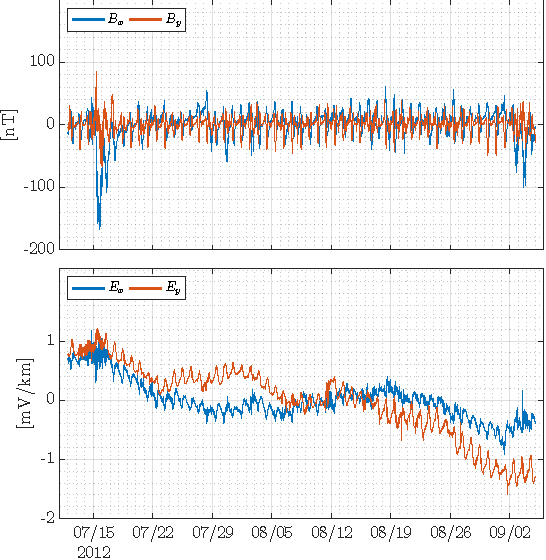
\includegraphics[width=\textwidth]{figures/tsplot-original-Middelpos-tf1.pdf}
  \caption{}
  \label{map}
\end{figure}

\section{Models and Methods}
\label{section:Models_and_Methods}

\begin{linenomath*}
  \begin{equation}
    G_o(t) = a_oE_x(t) + b_oE_y(t)
    \label{model1}
  \end{equation}
\end{linenomath*}

\noindent

\section{Model Evaluation}
\label{section:Model_Evaluation}

\section{Results}
\label{Results}

\section{Discussion}
\label{Discussion}

\section{Conclusions}

\clearpage

\section{Appendix}

\begin{table}
  \caption{Periods associated with evaluation frequency bands used for regression and smoothing spectra. \# is the evaluation frequency number, $N$ is the number of DFT points in the band, and $T_e\equiv 1/f_e$. The band range is from $T_l$ through $T_h$.}
  \centering
  \begin{tabular}{l l l l l}
    \hline \\
    \# & $N$ & $T_e$ [s] & $T_l$ [s] & $T_h$ [s] \\
    \hline \\
    1 & 2 & 43200 & 28800 & 86400 \\
    2 & 2 & 28800 & 21600 & 43200 \\
    3 & 3 & 21600 & 14400 & 43200 \\
    4 & 4 & 14400 & 9600 & 28800 \\
    5 & 5 & 10800 & 7200 & 21600 \\
    6 & 6 & 7854.5 & 5400 & 14400 \\
    7 & 8 & 5760 & 3927.3 & 10800 \\
    8 & 12 & 3927.3 & 2618.2 & 7854.5 \\
    9 & 16 & 2880 & 1920 & 5760 \\
    10 & 22 & 2009.3 & 1350 & 3927.3 \\
    11 & 31 & 1440 & 960 & 2880 \\
    12 & 43 & 1016.5 & 680.3 & 2009.3 \\
    13 & 61 & 720 & 480 & 1440 \\
    14 & 85 & 511.2 & 341.5 & 1016.5 \\
    15 & 120 & 361.5 & 241.3 & 720 \\
    16 & 170 & 255.6 & 170.4 & 511.2 \\
    17 & 240 & 180.8 & 120.5 & 361.5 \\
    18 & 338 & 128 & 85.4 & 255.6 \\
    19 & 478 & 90.5 & 60.3 & 180.8 \\
    20 & 676 & 64 & 42.7 & 128 \\
    21 & 956 & 45.2 & 30.2 & 90.5 \\
    22 & 1351 & 32 & 21.3 & 64 \\
    23 & 1910 & 22.6 & 15.1 & 45.2 \\
    24 & 2701 & 16 & 10.7 & 32 \\
    25 & 3819 & 11.3 & 7.5 & 22.6 \\
    26 & 5401 & 8 & 5.3 & 16 \\
    27 & 7638 & 5.7 & 3.8 & 11.3 \\
    28 & 10801 & 4 & 2.7 & 8 \\
    \hline \\
  \end{tabular}
  \label{evaluationperiods}
\end{table}

\clearpage

\bibliography{paper.bib}

\end{document}
